\newpage
\section{Auswertung}

In diesem Abschnitt wird der Versuch ausgewertet.

\subsection{Vorbereitungsaufgabe}
Als Vorbereitungsaufgabe für den Versuch wurden die Dopplerwinkel $\alpha$ zu den Prismenwinkel $\theta = 15° , 30°$ und $60°$ bestimmt.

\begin{table}
    \centering
    \caption{Prismenwinkel zu Dopplerwinkel}
    \begin{tabular}{c c}
        \toprule
        {$\theta$} & {$\alpha$}  \\
        \midrule
        15° & 80.064°  \\
        30° & 70.528°  \\
        60° & 54.735°  \\
        \bottomrule
    \end{tabular}
    \label{tab:vor}
\end{table}

\subsection{Bestimmung der Strömungsgeschwindigkeit}

Die aufgenommenen Messwerte bei den unterschiedlichen Rohr Innendurchmessern $d$ werden in die Tabelle (\ref{tab:a}) eingetragen, wobei k für den Dopplerwinkel steht.

\begin{table}
    \centering
    \caption{Messergebnisse der Dopplerverschiebung mit der Flussgeschwindigkeit $v_0$} 
    \begin{tabular}{c | c c c c}
        \toprule
        {$d \, \text{in} \, \si{\milli\meter} $} & {$v_0 \, / \, \si{\liter\per\minute}$} & {$\text{k bei 15°} \, / \, \si{\hertz}$} & {$\text{k  bei 30°} \, / \, \si{\hertz}$} & {$\text{k bei 60°} \, / \, \si{\hertz}$} \\
        \midrule
    7 &    2     &      55    &      195   &      378    \\
     &    3      &     146    &     342    &     647   \\
     &    4      &     244    &     525    &     989   \\
     &    5      &     354    &     732    &     1385   \\
     &    6      &     452    &     964    &     1843   \\
     &    7.5    &     647    &     1367   &     2515   \\
    \midrule 
    10 &    2     &      -49  &       85     &     -122 \\
     &    3       &    -73    &     134      &   -220 \\
     &    4       &    -110   &     208      &   -342 \\
     &    5       &    -146   &     305      &   -464 \\
     &    6       &    -183   &     403      &   -647 \\
     &    7.5     &    -256   &     598      &   -879 \\
    \midrule 
    16 &    2      &     49  &        49   &       61 \\
     &    3        &   61    &      73     &     122 \\
     &    4        &   73    &      110    &     183 \\
     &    5        &   98    &      134    &     256 \\
     &    6        &   110   &      171    &     342 \\
     &    7.5      &   171   &      256    &     500 \\
        \bottomrule
    \end{tabular}
    \label{tab:a}
\end{table}

\noindent
Mithilfe der Formel (\ref{equ:Geschw}) und der verwendeten Ultraschallsonde mit $\nu_0 = 2 \si{\mega\hertz} $ lässt sich die Strömungsgeschwindigkeit $\nu$, sowie der Winkel $\alpha$ bestimmen. Diese werden in die Tabelle (\ref{tab:b}) eingetragen.

\begin{equation}
    \label{equ:Geschw}
    v = \frac{\increment \nu \cdot c}{2\nu \cdot cos(\alpha)}
\end{equation}


\begin{table}
    \centering
    \caption{Berechnete Flussgeschwindigkeit $v_0$ in Abhängigkeit des Winkels}
    \begin{tabular}{c | c c c c}
        \toprule
        {$d \, \text{in} \, \si{\milli\meter} $} & {$v_0 \, \text{in} \, \si{\liter\per\minute}$} & {$\nu \,\text{ bei } 15° \, \text{in} \, \si{\meter\per\second}$} & {$\nu \, \text{ bei } 30° \, \text{in} \, \si{\meter\per\second}$} & {$\nu \, \text{ bei } 60° \, \text{in} \, \si{\meter\per\second}$} \\
        \midrule
    7 &    2     &     0.143    &     0.263   &     0.294 \\
     &    3      &     0.380    &     0.461   &     0.504 \\
     &    4      &     0.636    &     0.708    &    0.770 \\
     &    5      &     0.923   &      0.988   &     1.079 \\
     &    6      &     1.178    &     1.301   &     1.436 \\
     &    7.5    &     1.687    &     1.845   &     1.960\\
    \midrule
    10 &    2     &    -0.127  &      0.114     &   -0.095  \\
     &    3       &    -0.190    &    0.180     &   -0.171  \\
     &    4       &    -0.286   &     0.280     &   -0.266  \\
     &    5       &    -0.380   &     0.411      &  -0.361  \\
     &    6       &    -0.477   &     0.544      &  -0.504  \\
     &    7.5     &    -0.667   &     0.807     &   -0.685 \\
    \midrule
    16 &    2      &   0.127  &       0.066   &     0.047  \\
     &    3        &   0.159    &     0.098    &    0.095 \\
     &    4        &   0.190    &     0.148   &     0.142 \\
     &    5        &   0.255    &     0.180   &     0.199 \\
     &    6        &   0.286   &      0.230    &    0.266 \\
     &    7.5      &   0.445   &      0.345   &     0.389 \\

        \bottomrule
    \end{tabular}
    \label{tab:b}
\end{table}

\noindent
In den folgenden Grafiken ist $\frac{\increment \nu}{cos(\alpha)}$ gegen die Strömungsgeschwindigkeit, für alle drei Rohr Innendurchmesser, aufgetragen.

\begin{figure}
    \centering
    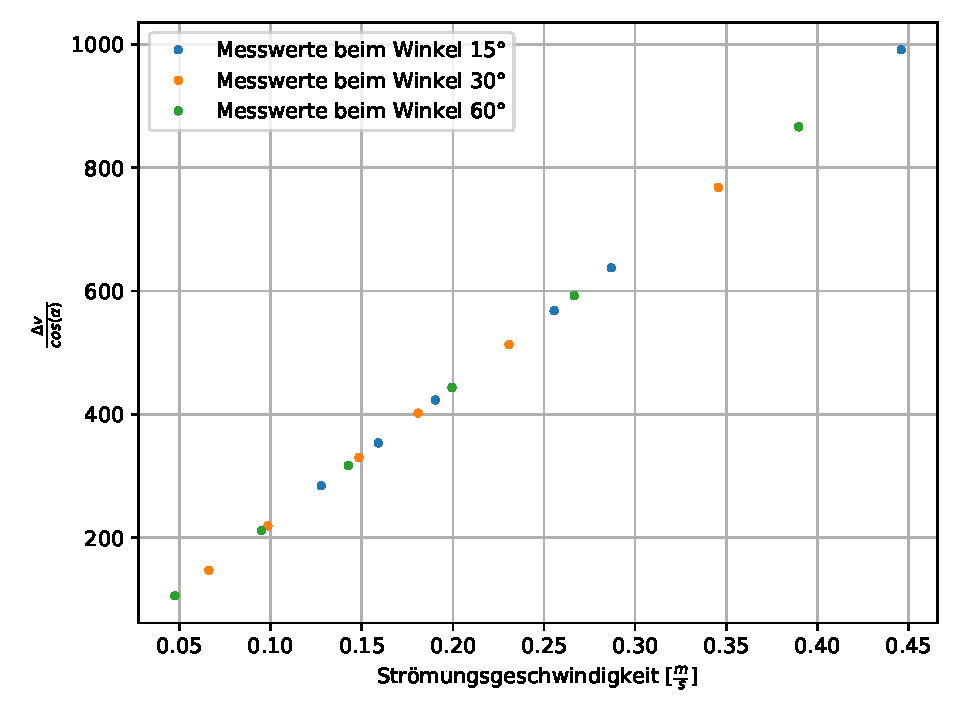
\includegraphics{Daten/7mm.pdf}
    \caption{Innendurchmesser von 7mm.}
    \label{fig:KeineAhnung}
\end{figure}

\begin{figure}
    \centering
    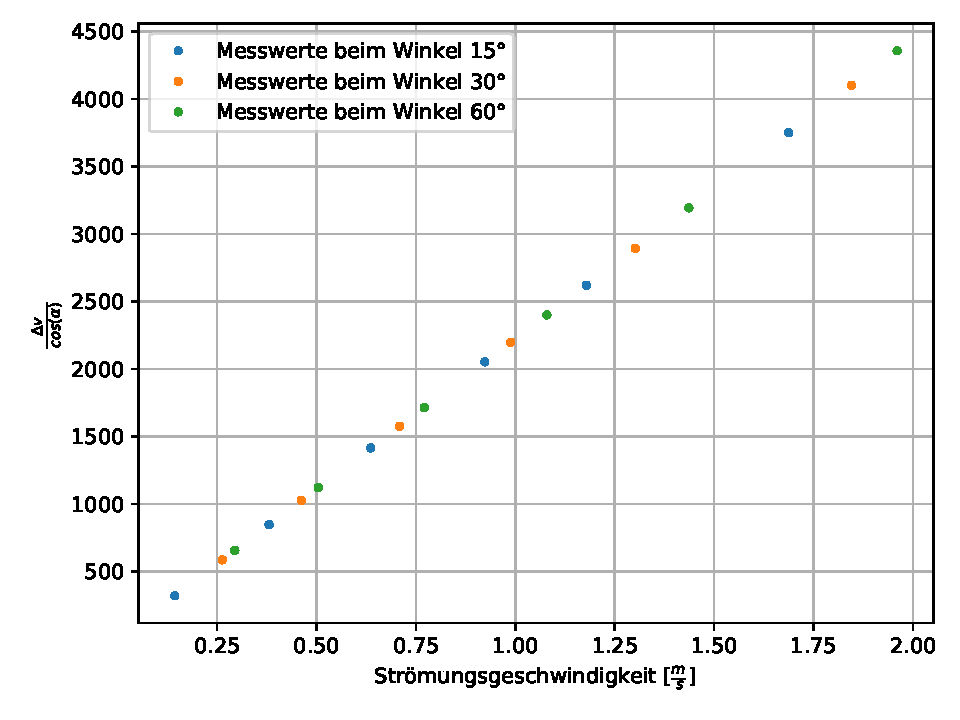
\includegraphics{Daten/10mm.pdf}
    \caption{Innendurchmesser von 10mm.}
    \label{fig:KeineAhnung}
\end{figure}
\begin{figure}
    \centering
    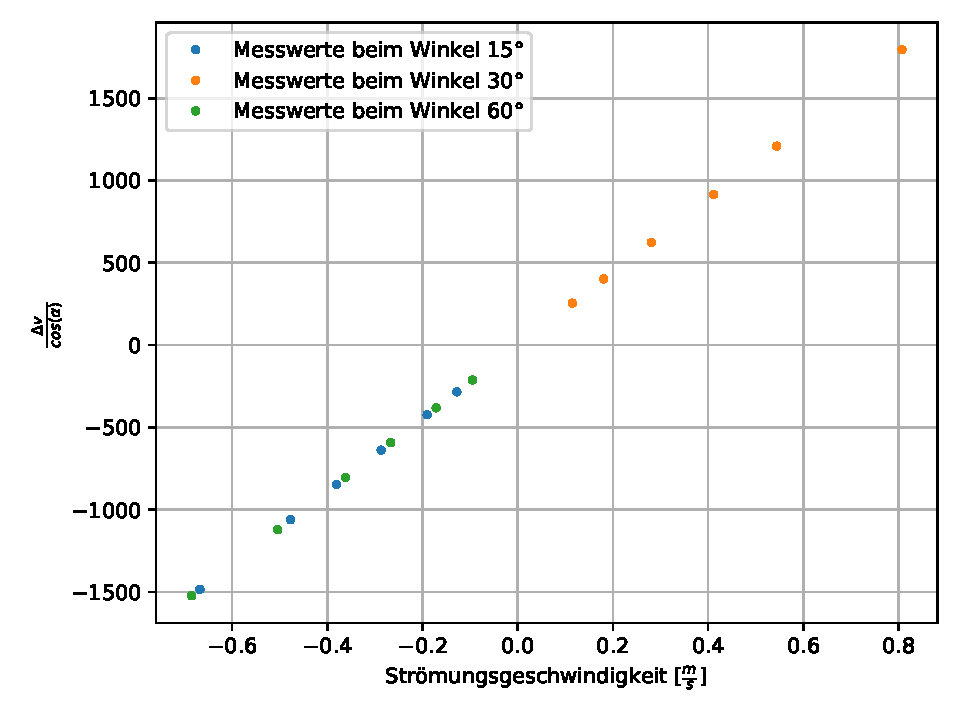
\includegraphics{Daten/16mm.pdf}
    \caption{Innendurchmesser von 16mm.}
    \label{fig:KeineAhnung}
\end{figure}



\subsection{Erstellung eines Strömungsprofil}

\noindent
Nun wird um das Strömungsprofil zu untersuchen, bei einem Prismenwinkel von $\theta$ = 15° gemessen. Einmal bei einer Leistung von 70\% und einmal bei einer Leistung von 45\%.
Das entspricht etwas einer Flussgeschwindigkeit von $5,3$ und $3,4 \, \si{\liter\per\minute}$. Alle Messwerte mit dem Index 1 sind bei $5,3 \, \si{\liter\per\minute}$ und 
alle Messwerte mit dem Index 2 sind bei $3,4 \, \si{\liter\per\minute}$ gemessen worden. Daraus folgt die Tabelle (\ref{tab:profil}).

\begin{table}
    \centering
    \caption{Messwerte des Strömungsprofils}
    \begin{tabular}{c c c c c}
        \toprule

       {$\text{Tiefe}\, / \, \si{\micro\second}$} & {$\nu _1\, / \, \si{\hertz}$}& { $I_1 \, / \, 100\si{\volt\squared\per\second} $} & {$\nu_2 \, / \, \si{\hertz}$} & {$I_2 \, / \, 100\si{\volt\squared\per\second}$}\\
        \midrule
        13         &     -171    &        60   & -98   & 55  \\
        13.5       &     -220    &        90   & -110  & 70  \\
        14         &     -244    &        100  & -122  & 87  \\
        14.5       &     -256    &        100  & -134  & 97  \\
        15         &     -269    &        104  & -146  & 120  \\
        15.5       &     -256    &        100  & -134  & 114  \\
        16         &     -232    &        105  & -122  & 116  \\
        16.5       &     -195    &        101  & -110  & 88  \\
        17         &     -159    &        90   & -98    & 49  \\
        17.5       &     -134    &        60   & 0      & 0  \\
        \bottomrule
    \end{tabular}
    \label{tab:profil}
\end{table}

\noindent
Nun kann für beide Flussgeschwindigkeit in je einem Diagramm die Streuintensität $I_x$ und die Momentangeschwindigkeit $v$, welche sich äquivalent, wie in der vorherigen 
Teilauswertung, als Funktion der Messtiefe aufgetragen werden. Daraus folgen die Grafiken (\ref{fig:1},\ref{fig:2}).

\begin{figure}
    \centering
    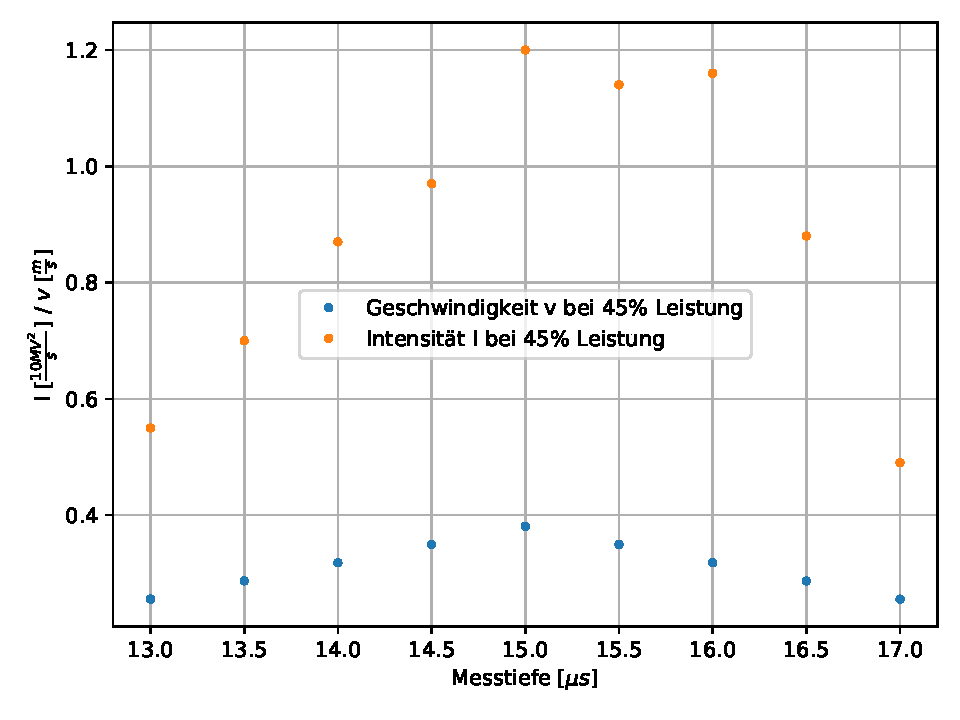
\includegraphics[width=\textwidth]{Daten/45.pdf}
    \caption{Plot bei einer Leistung von 45\%}
    \label{fig:1}
\end{figure}

\begin{figure}
    \centering
    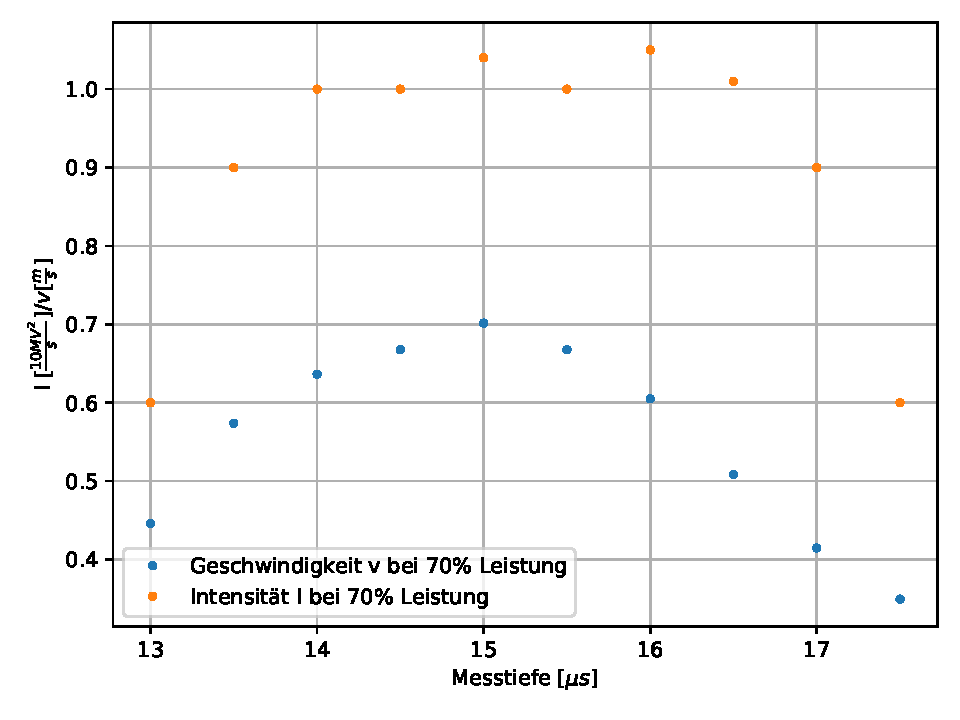
\includegraphics[width=\textwidth]{Daten/70.pdf}
    \caption{Plot bei einer Leistung von 70\%}
    \label{fig:2}
\end{figure}

